
In this section we motivate precision measurements on the tensor structures of one Higgs couplings with two electroweak gauge bosons (HVV) and two Higgses couplings with two electroweak gauge bosons (HHVV) in HE/HL LHC. There exist special relations between HVV and HHVV couplings in composite Higgs models that are universal, independent of the  symmetry breaking pattern invoked in a particular model. These "universal relations" are controlled by a single input parameter, the decay constant $f$ of the pseudo-Nambu-Goldstone Higgs boson. Testing the universal relations requires measuring the tensor structures of HVV and HHVV couplings to high precision.  In particular,  HHVV interactions remains as one of the few untested predictions of the Standard Model Higgs boson, which can be probed through the double Higgs production in the vector boson fusion (VBF) channel at the LHC. Below we summarise the main results. The phenomenological details and theoretical foundation can be found in Refs.~\cite{Low:2014nga,Low:2014oga,Liu:2018vel,Liu:2018qtb}


%\section{HVV and HHVV Couplings in Composite Higgs Models}

At the leading two-derivative order, the HVV and HHVV couplings in composite Higgs models in the unitary gauge is given by the following simple expression:
\begin{equation}
\label{eq:twod}
{\cal L}^{(2)} = \frac12 \partial_\mu h\partial^\mu h+\frac{g^2f^2}{4}\sin^2\left(\theta+h/f\right)\left(W_\mu^+W^{-\, \mu}+\frac1{2\cos^2\theta_W}Z_\mu Z^\mu\right)\ ,
\end{equation}
where  $v=246$ \UGeV, $f$ is the decay constant of the composite Higgs boson and $\sin\theta=v/f$. This result is independent of the symmetry breaking pattern of the strong composite sector in the UV, apart from the overall normalisation of $f$, which does depend on the UV model.

At the four-derivative level, we parametrise the HVV and HHVV couplings  as follows:
\begin{equation}
\label{eq:Cis}
{\cal L}^{(4)} =  \sum_i\frac{m_W^2}{m_\rho^2} \left(C^h_i {\cal I}^h_i  +C^{2h}_i {\cal I}^{2h}_i\right) ,
\end{equation}
where the definition of the  operators ${\cal I}^h_i$ and ${\cal I}^{2h}_i$ are presented in Table~\ref{tab:oneh} and Table~\ref{tab:twoh}. On the other hand, $C^h_i$ and $C^{2h}_i$ are Wilson coefficients which depend on six unknowns ($\theta, c_3, c_4^\pm, c_5^\pm$) in composite Higgs models and on four unknowns ($c_W, c_B, c_{HW}, c_{HB}$)  in the Standard Model Effective Field Theory (SMEFT). In the above $m_\rho=g_\rho f$ is the typical mass scale of the new composite resonances. The different Lorentz structures lead to different angular distributions in the decay products and, therefore, can be measured accordingly. At the LHC Run 1,  testing the tensor structure of HVV couplings was among the top priorities and gave confidence to the Higgs nature of the 125 \UGeV resonance. (See, for example, Ref.~\cite{Sirunyan:2017tqd}.) A similar program for HHVV coupling is currently lacking and should be pursued at HE/HL LHC.

%%%%%%%%%%%%%%%%%%%%%%%%%%%%%%%%%%%%%%%%
\begin{table}[!t]
\begin{center}
\caption{Single Higgs coupling coefficients $C_i^h$ for the non-linearity case (NL) and the  purely dimension-6 contributions (D6) in SMEFT. Here  $c_w, t_w$ and $c_\theta$ denote $\cos\theta_W, \tan\theta_W$ and $\cos\theta$, respectively, where $\theta_W$ is the weak mixing angle. ${\cal D}^{\mu\nu}$ denotes $\partial^\mu \partial^\nu - \eta^{\mu\nu} \partial^2$. Hermitian conjugate of an operator is implied when necessary.}\label{tab:oneh}
\begin{tabular}{lc c c c ccc}\hline\hline
${\cal I}^{h}_i$ &   $  C^h_i$ (NL)& $  C^h_i$ (D6)\\
 \hline
(1) $  \frac{h}{v} Z_{\mu} {\mathcal{D}}^{\mu \nu} Z_{\nu}$ & $ \frac{4 c_{ 2 w} }{c^2_{w}}  (-2 c_3  + c_4^- )  
+\frac{4}{c^2_{w}}   c_4^+ c_\theta $ &$ 2 (c_W + c_{HW}) +2 t^2 _{w} (c_B + c_{HB})$\\
 %\hline
(2)  $ \frac{h}{v}  Z_{\mu\nu} Z^{\mu\nu}$ & $  -\frac{2  c_{2 w}}{c^2_{w}}  ( c_4^-  + 2 c_5^- ) -\frac{2 }{c^2_{w}}   ( c_4^+  - 2 c_5^+ ) c_\theta    $&$-( c_{HW} + t^2_{w} c_{HB})$\\
 %\hline
(3)  $ \frac{h}{v}  Z_{\mu} {\mathcal{D}}^{\mu \nu} A_{\nu}$ & $8  ( - 2 c_3  +   c_4^- )  t_{ w} $& $ 2 t_w (c_W + c_{HW}-c_B - c_{HB})  $ \\
%\hline
(4) $ \frac{h}{v}  Z_{\mu\nu} A^{\mu\nu}$ & $-4  (  c_4^-   +2 c_5^- )  t_{ w} $&  $ -  t_w(c_{HW}- c_{HB})$\\
%\hline
(5)  $ \frac{h}{v}  W^+_{\mu} {\mathcal{D}}^{\mu \nu} W^-_{\nu}$ & $4 (-2 c_3  + c_4^- ) 
+  4 c_4^+ c_\theta $ & $2 (c_W + c_{HW})$\\
 %\hline
(6) $ \frac{h}{v}  W^+_{\mu\nu} W^{-\mu\nu} $ & $ -4( c_4^- + 2 c_5^-)   -4 ( c_4^+  - 2 c_5^+) c_\theta $&   $-2 c_{HW} $ \\
\hline\hline
\end{tabular}
\end{center}
\end{table}

%%%%%%%%%%%%%%%%%%%%%%%%%%%%%%%%%%%%%%%%
\begin{table}[!h]
\begin{center}
\caption{The coupling coefficients $C_i^{2h}$ involve two Higgs bosons  for universal  non-linearity case (NL) and the  dimension-six case in SMEFT (D6). A cross ($\times$) means there is no contribution at the order we considered. Notice $C_i^{2h}=C_i^h/2$ for  SMEFT at the dimension-6 level. $c_{2\theta}$ and $s_\theta$ denote $\cos 2\theta$ and $\sin\theta$, respectively.}\label{tab:twoh}
\begin{tabular}{c c c c c}
\hline\hline
${\cal I}^{ 2 h}_i$ &  $ C^{ 2h}_i$ (NL) &  $   C^{2h}_i$ (D6) \\
 \hline
(1) $  \frac{h^2}{v^2} Z_{\mu} {\mathcal{D}}^{\mu \nu} Z_{\nu}$ & $ \frac{2c_{ 2 w} }{c^2_{w}} ( - 2 c_3  +  c_4^-  ) c_\theta   +   \frac{2 }{c^2_{w}} c_4^+ c_{2 \theta}  $ & $\frac12 C_1^h$ 
 \\
 %\hline
(2) $  \frac{h^2}{v^2} Z_{\mu\nu} Z^{\mu\nu}$ & $ - \frac{c_{2 w}}{c^2_{w}}  (c_4^-  + 2 c_5^-  ) c_\theta   - \frac{1}{c^2_{w}}  (c_4^+ - 2 c_5^+ ) c_{2 \theta}   $ &$\frac12 C_2^h$ \\
 %\hline
(3) $  \frac{h^2}{v^2} Z_{\mu} {\mathcal{D}}^{\mu \nu} A_{\nu}$ & $ 4  t_{ w}  ( -2c_3   + c_4^- ) c_\theta $ & $\frac12 C_3^h$ \\
 %\hline
(4) $  \frac{h^2}{v^2} Z_{\mu\nu} A^{\mu\nu}$ & $ -2  t_{ w}   (   c_4^-  + 2 c_5^-  )  c_\theta $ &   $\frac12 C_4^h$  \\
   % \hline
(5)  $ \frac{h^2}{v^2} W^+_{\mu} {\mathcal{D}}^{\mu \nu} W^-_{\nu}$ & $ 2  (- 2c_3 + c_4^- ) c_\theta  + 2 c_4^+ c_{2 \theta}   $ & $\frac12 C_5^h$ \\
 %\hline
(6) $ \frac{h^2}{v^2} W^+_{\mu\nu} W^{-\mu\nu}$ & $  -2 ( c_4^- + 2 c_5^- )c_\theta   -2  (c_4^+  - 2 c_5^+ ) c_{2\theta}  $ &  $\frac12 C_6^h$\\
%\hline
(7) $      \frac{(\partial_\nu h)^2} {v^2}Z_\mu Z^{ \mu}  $& $\frac{8 }{c^2_{w}}  c_1 s^2_\theta$ &  $\times$\\
%\hline
(8)  $   \frac{\partial_\mu h \partial_\nu h}{v^2} \, Z^\mu Z^\nu  $& $\frac{8 }{c^2_{w}}  c_2  s^2_\theta$&  $\times$\\
%\hline
(9) $      \frac{(\partial_\nu h)^2}{v^2} W^+_\mu W^{- \mu}  $& $16 c_1 s^2_\theta$ & $\times$ \\
%\hline
(10) $  \frac{ \partial^\mu h \partial^\nu h }{v^2}\, W^+_{\mu} W^{-}_\nu  $& $16  c_2  s^2_\theta$ &  $\times$\\
\hline\hline
\end{tabular}
\end{center}
\end{table}
%%%%%%%%%%%%%%%%%%%%%%%%%%%%%%%%%%%%%%%%



In general, we have two different Lorentz structure in the HVV couplings:
\begin{equation}
\label{eq:lstruc1}
\frac{h}{v} V_{1\,\mu} \mathcal{D}^{\mu\nu} V_{2\,\nu} \ ,\qquad \frac{h}{v} V_{1\,\mu\nu}  V_2^{\mu\nu} \ ,
\end{equation}
where  ${\mathcal{D}}^{\mu\nu} = \partial^\mu\partial^\nu-\eta^{\mu\nu}\partial^2$ and $V_{1,2} \in\{W, Z,\gamma\}$ with electric charge conservation implicitly indicated. For HHVV couplings we have: 
\begin{equation}
\frac{h^2}{v^2} V_{1\,\mu} {\mathcal{D}}^{\mu\nu} V_{2\,\nu}\ , \quad  \frac{h^2}{v^2} V_{1\,\mu\nu}  V_2^{ \mu\nu} \ , \qquad \frac{\partial_\mu h \partial_\nu h}{v^2} V_1^\mu V_2^{\nu}, \qquad \frac{\partial_\mu h \partial^\mu h}{v^2} V_1^\mu V_{2\mu} \ .
\label{eq:lstruc2}
\end{equation}
The ultimate goal then will be to measure these different tensor structures at CLIC.

From Table~\ref{tab:oneh} and Table~\ref{tab:twoh}, we can extract relations among $C_i^{h}$ and $C_i^{2h}$ that only depend on the $\theta$. We call them "universal relations" as they represent universal predictions of a composite Higgs boson, whose nonlinear interactions are dictated by the underlying shift symmetries acting on the four components of the Higgs doublet \cite{Low:2014nga,Low:2014oga,Liu:2018vel,Liu:2018qtb}.  Some examples of universal relations involving both HVV and HHVV couplings are:
\begin{eqnarray}
\label{eq:ident3}
&& \frac{C^{2h}_3}{C^h_3} = \frac{C^{2h}_4}{C^h_4} =\frac12 \cos\theta  \ ,\\
\label{eq:ident4}
&& \frac{C^{2h}_5 - C^{2h}_3 /2t_w} {C^h_5 - C^{h}_3/2t_{w}} =  \frac{C^{2h}_6 -C^{2h}_4/t_{w} }{C^h_6 - C^{h}_4/t_{w}} = \frac{\cos2\theta}{2\cos\theta} \approx \frac12\left(1 - \frac32 \xi \right)\, ,\\
&&\frac{s_{2w} \,C^{2h}_1 - c_{2w}\,   C^{2h}_3} {s_{2w}\, C^h_1-c_{2w} \,  C^{h}_3} =\frac{s_{2w}\, C^{2h}_2 - c_{2w}\,   C^{2h}_4} {s_{2w}\, C^h_2-c_{2w}\,   C^{h}_4}  = \frac{\cos2\theta}{2\cos\theta}\approx \frac12\left(1 - \frac32 \xi \right)\ .
\end{eqnarray}
These relations depend on one single parameter $\theta$ or, equivalently, $\xi=v^2/f^2$. In other words, they can be used to over-constrain the parameter $f$. If the 125 \UGeV Higgs boson indeed arises as a pseudo-Nambu-Goldstone boson, the decay constant $f$ as measured from the different universal relations must be consistent with one another.





%\section{VBF and Associated HH Productions at the LHC}

In order to test the universal relations, it is necessary to measure the tensor structures of HHVV couplings. This is where the HE/HL LHC could have an advantage over circular lepton colliders. At a hadron collider, $C^h_i$ can be measured from single Higgs decays into four leptons in a fashion similar to the analysis performed in Ref.~\cite{Sirunyan:2017tqd}, while measurements on $C^{2h}_i$ would have to rely on double Higgs production in the VBF  channel and the associated production with a $Z$ boson. The production topology is displayed in Fig.~\ref{fig:testhh}.


\begin{figure}[!t]
\centering
    \subfloat[Double Higgs production through vector boson fusion.]{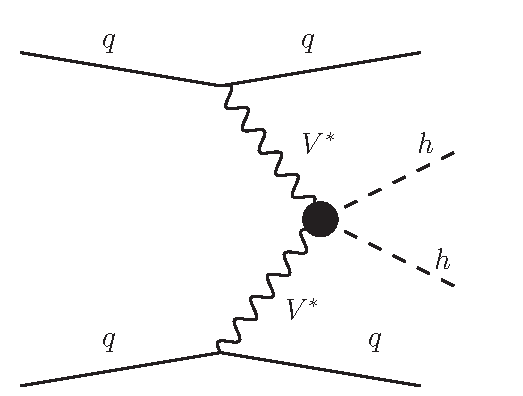
\includegraphics[height=3.3cm]{\main/section4/plots/fdhh_vbf.pdf}}
  \quad \ \ %\hfill
  \subfloat[Double Higgs production in association with a vector boson.]{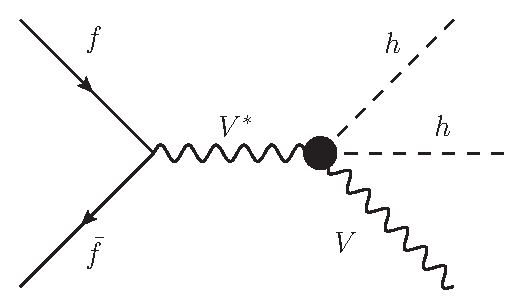
\includegraphics[height=2.8cm]{\main/section4/plots/fdhh_apv.pdf}}
 % \quad \ \ %\hfill
 % \subfloat[Off-shell Single Higgs decay.]{\includegraphics[height=3.3cm]{./figures/fdhh_ohd.pdf}}
%   \quad \ \ %\hfill
  \caption{Production and decay topology of venues to test the HHVV couplings at the LHC. A black dot represents contributions from various Feynman diagrams. \label{fig:testhh}}
\end{figure}
%%%%%%%%%%%%%%%%%%%%%%%%%%%%%%%%%%%%%%%%
%We have derived the universal relations in the composite Higgs models involving the HVV, HHVV,(H)VVV couplings. Our construction only relies on the IR-date: Alder's zero condition and the unbroken $SO(4)$.  The HVV and VVV couplings have been studied extensively in the literature, while it is not the case for HHVV, in particular the different Lorentz structures. In Fig.~\ref{fig:testhh}, we have shown different ways of measuring $HHVV$ couplings including  the double Higgs production in the vector boson fusion (VBF) channel, the  double Higgs production in association with a vector boson and even an off-shell single Higgs decay: $h^* \rightarrow h^* V^* V$. 



In Fig.~\ref{fig:xshh}  we show the double Higgs production rate in the VBF channel and the associated production channel in a hadron collider as a function of the centre-of-mass energy $\sqrt{S}$, adopting the computation done in Ref.~\cite{Frederix:2014hta}. The VBF rate at 13 \UTeV is less than 1 fb, while at 27 \UTeV the cross-section is about 3 fb, which offers the best chance to probe the HHVV couplings at the LHC. 

\begin{figure}[!t]
\centering
   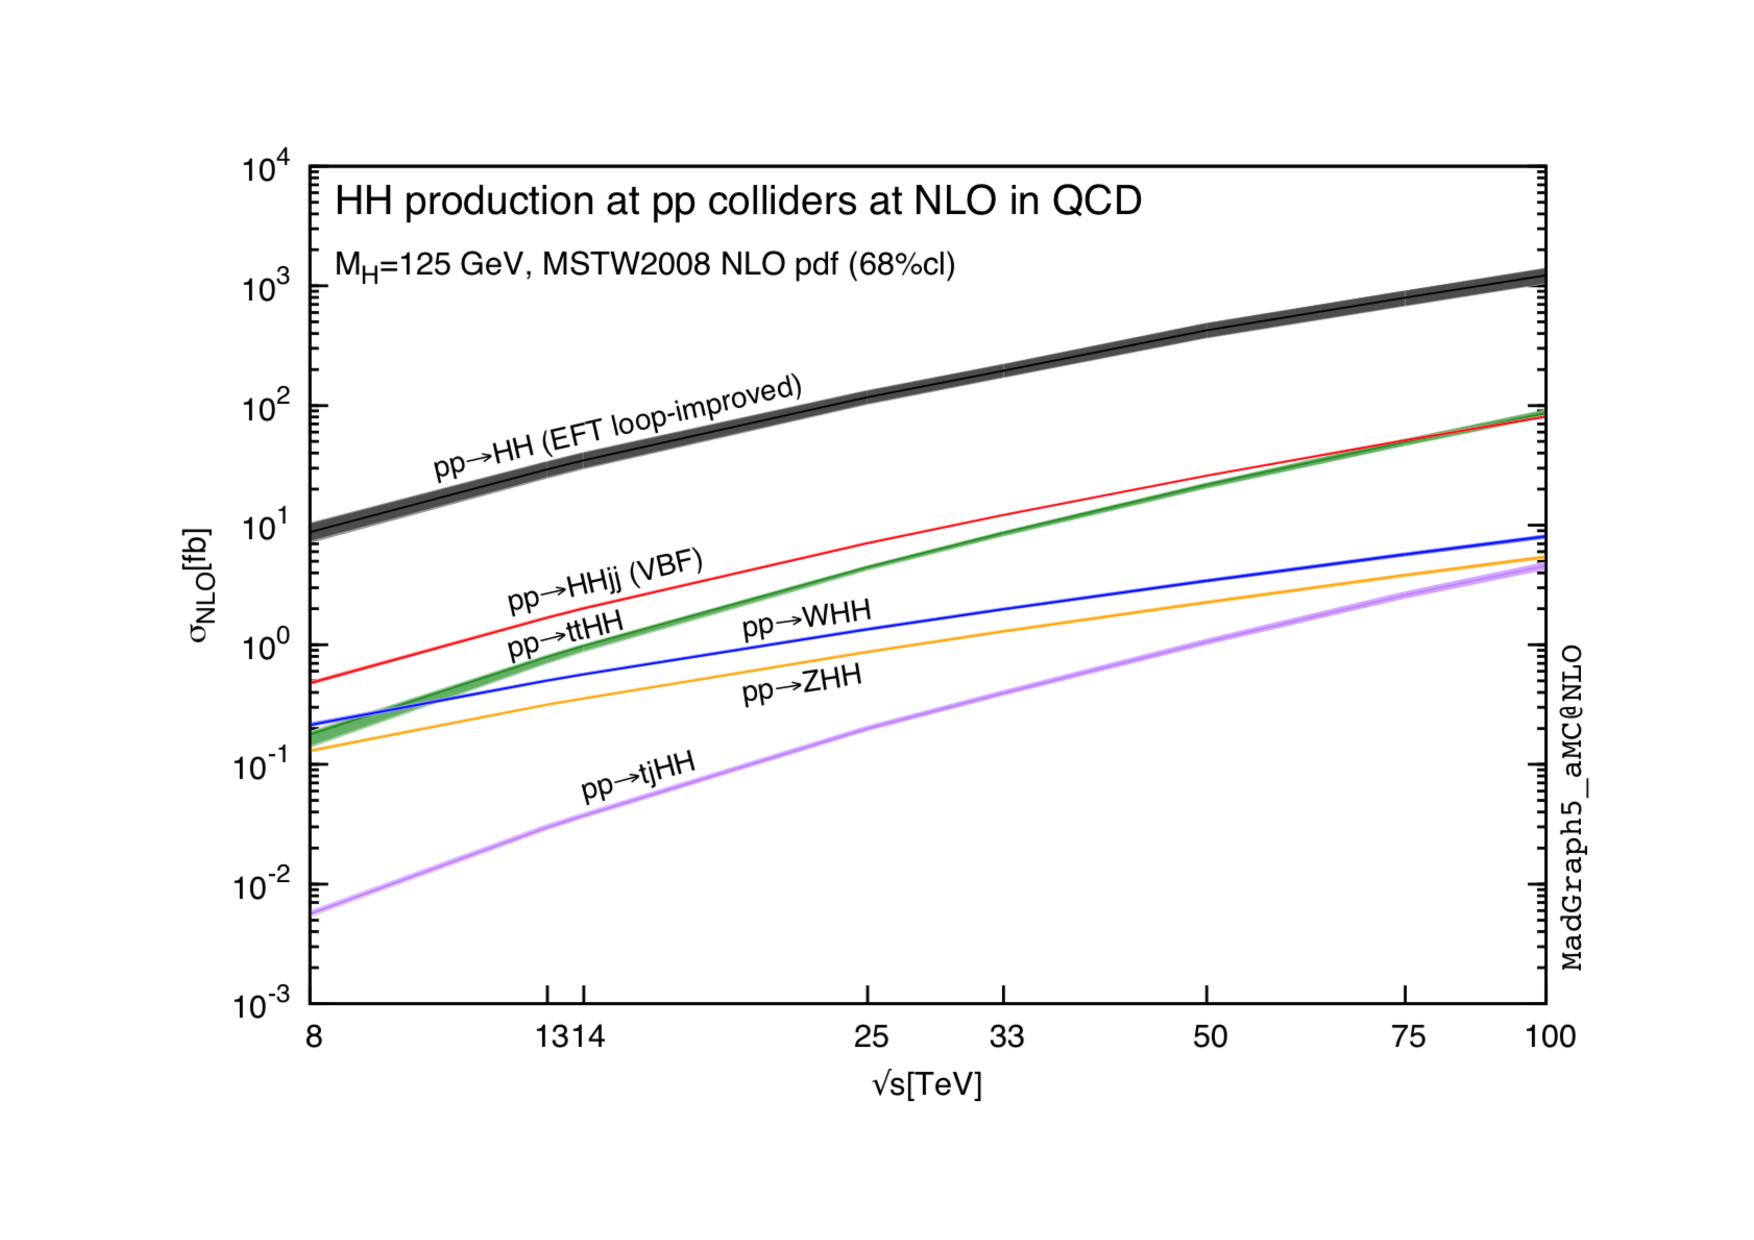
\includegraphics[width=9cm]{\main/section4/plots/ppxshh.pdf}
  \caption{Double Higgs production rates, including the VBF  and associate production channels, at a hadron collider. This figure is adopted from Ref.~\cite{Frederix:2014hta}. \label{fig:xshh}}
\end{figure}


The analysis of the HHVV coupling is further discussed in the next section \ref{sec:VVHHcont}.
%For a CM energy below roughly 1.2 TeV, the associate production dominates over the $WW$ fusion. However, in the high energy regime, the WW fusion production rate rises continually, reaching 0.9 fb for $\sqrt{S}=3$ TeV. As a comparison, at $\sqrt{S}=1$ TeV the associate production rate is about 0.1 fb. This demonstrates that a 3 TeV CLIC is a unique machine to probe the HHVV coupling structure.





